%%%%%%%%%%%%%%%%%%%%%%%%%%%%%%%%%%%%%%%%%%%%%%%%%%%%%%%%%%%%%%%%%%%%%%%%%%%%%%%%%%%%%%%
%%%%%%%%%%%%%%%%%%%%%%%%%%%%%%%%%%%%%%%%%%%%%%%%%%%%%%%%%%%%%%%%%%%%%%%%%%%%%%%%%%%%%%%
% 
% This top part of the document is called the 'preamble'.  Modify it with caution!
%
% The real document starts below where it says 'The main document starts here'.

\documentclass[12pt]{article}
\usepackage{graphicx}
\usepackage{float}
\usepackage{amssymb,amsmath,amsthm}
\usepackage[top=1in, bottom=1in, left=1.25in, right=1.25in]{geometry}
\usepackage{fancyhdr}
\usepackage{enumerate}

% Comment the following line to use TeX's default font of Computer Modern.
\usepackage{times,txfonts}

\newtheoremstyle{homework}% name of the style to be used
  {18pt}% measure of space to leave above the theorem. E.g.: 3pt
  {12pt}% measure of space to leave below the theorem. E.g.: 3pt
  {}% name of font to use in the body of the theorem
  {}% measure of space to indent
  {\bfseries}% name of head font
  {:}% punctuation between head and body
  {2ex}% space after theorem head; " " = normal interword space
  {}% Manually specify head
\theoremstyle{homework} 

% Set up an Exercise environment and a Solution label.
\newtheorem*{exercisecore}{Exercise \@currentlabel}
\newenvironment{exercise}[1]
{\def\@currentlabel{#1}\exercisecore}
{\endexercisecore}

\newcommand{\localhead}[1]{\par\smallskip\noindent\textbf{#1}\nobreak\\}%
\newcommand\solution{\localhead{Solution:}}

%%%%%%%%%%%%%%%%%%%%%%%%%%%%%%%%%%%%%%%%%%%%%%%%%%%%%%%%%%%%%%%%%%%%%%%%
%
% Stuff for getting the name/document date/title across the header
\makeatletter
\RequirePackage{fancyhdr}
\pagestyle{fancy}
\fancyfoot[C]{\ifnum \value{page} > 1\relax\thepage\fi}
\fancyhead[L]{\ifx\@doclabel\@empty\else\@doclabel\fi}
\fancyhead[C]{\ifx\@docdate\@empty\else\@docdate\fi}
\fancyhead[R]{\ifx\@docauthor\@empty\else\@docauthor\fi}
\headheight 15pt

\def\doclabel#1{\gdef\@doclabel{#1}}
\doclabel{Use {\tt\textbackslash doclabel\{MY LABEL\}}.}
\def\docdate#1{\gdef\@docdate{#1}}
\docdate{Use {\tt\textbackslash docdate\{MY DATE\}}.}
\def\docauthor#1{\gdef\@docauthor{#1}}
\docauthor{Use {\tt\textbackslash docauthor\{MY NAME\}}.}
\makeatother

% Shortcuts for blackboard bold number sets (reals, integers, etc.)
\newcommand{\Reals}{\ensuremath{\mathbb R}}
\newcommand{\Nats}{\ensuremath{\mathbb N}}
\newcommand{\Ints}{\ensuremath{\mathbb Z}}
\newcommand{\Rats}{\ensuremath{\mathbb Q}}
\newcommand{\Cplx}{\ensuremath{\mathbb C}}
%% Some equivalents that some people may prefer.
\let\RR\Reals
\let\NN\Nats
\let\II\Ints
\let\CC\Cplx

%%%%%%%%%%%%%%%%%%%%%%%%%%%%%%%%%%%%%%%%%%%%%%%%%%%%%%%%%%%%%%%%%%%%%%%%%%%%%%%%%%%%%%%
%%%%%%%%%%%%%%%%%%%%%%%%%%%%%%%%%%%%%%%%%%%%%%%%%%%%%%%%%%%%%%%%%%%%%%%%%%%%%%%%%%%%%%%
% 
% The main document start here.

% The following commands set up the material that appears in the header.
\doclabel{Stat 300: Homework 7}
\docauthor{Stefano Fochesatto}
\docdate{\today}

\begin{document}

\begin{exercise}{4.68} "The special case..."  (Note that this problem is just a special case of the Gamma distribution, so you can do parts a, b using the Gamma distribution. For part (b) you can use R, then pgamma(30,shape=alpha, scale=beta).\\

  \begin{enumerate}
    \item  What is the expected value of X? If the time (in minutes)  between  arrivals  of  successive  customers  is  exponentially  distributed  with  $\lambda = 5.5$,  how  much  time can be expected to elapse before the tenth customer arrives?\\
    
    \solution Since the Erlang distribution is a special case of the gamma, and we know the expected value for the gamma we simply plug in,
    $X \sim Gamma(10, .5)$,
    \begin{equation*}
      E(x) = \alpha\beta = n \dfrac{1}{\lambda} = 10(2) = 20.
    \end{equation*}
    \vspace{.25in}
  


    \item If customer interarrival time is exponentially distributed  with  $\lambda = .5$,  what  is  the  probability  that  the  tenth  customer  (after  the  one  who  has  just  arrived)  will arrive within the next 30 min?\\
    
    \solution Simply computing (with R) the $P(X\le 30)$ where $X \sim Exp(10, .5)$,
    \begin{equation*}
      P(X\le 30) = 0.9301463.
    \end{equation*}
    
  \end{enumerate}

\end{exercise}
\vspace{.5in}




\begin{exercise}{Supplimental 1} We have a data set consisting of grass cover in n = 10 plots:  c(0.34, 0.3, 0.9, 0.89, 0.34, 0.72, 0.61, 0.84, 0.17, 0.41).  Of the distributions discussed in section 4.6 (Weibull, Lognormal, Beta), which is probably a better choice of model for this data?  Why?\\

  
\solution Since the grass coverage is measured as a percentage, ie (0 - 1) it's most definitely going to be a beta distribution that best models the data. also in most cases id imagine 
that grass coverage is fairly uniform (depending on the season of course) where the beta function gives the flexibility to model something close to the uniform. 

\end{exercise}
\vspace{.5in}




\begin{exercise}{4.88} (This technique is a good way to check the normality of a data set)\\
  \solution Using $R$ to plot the probability plot,
\begin{center}
	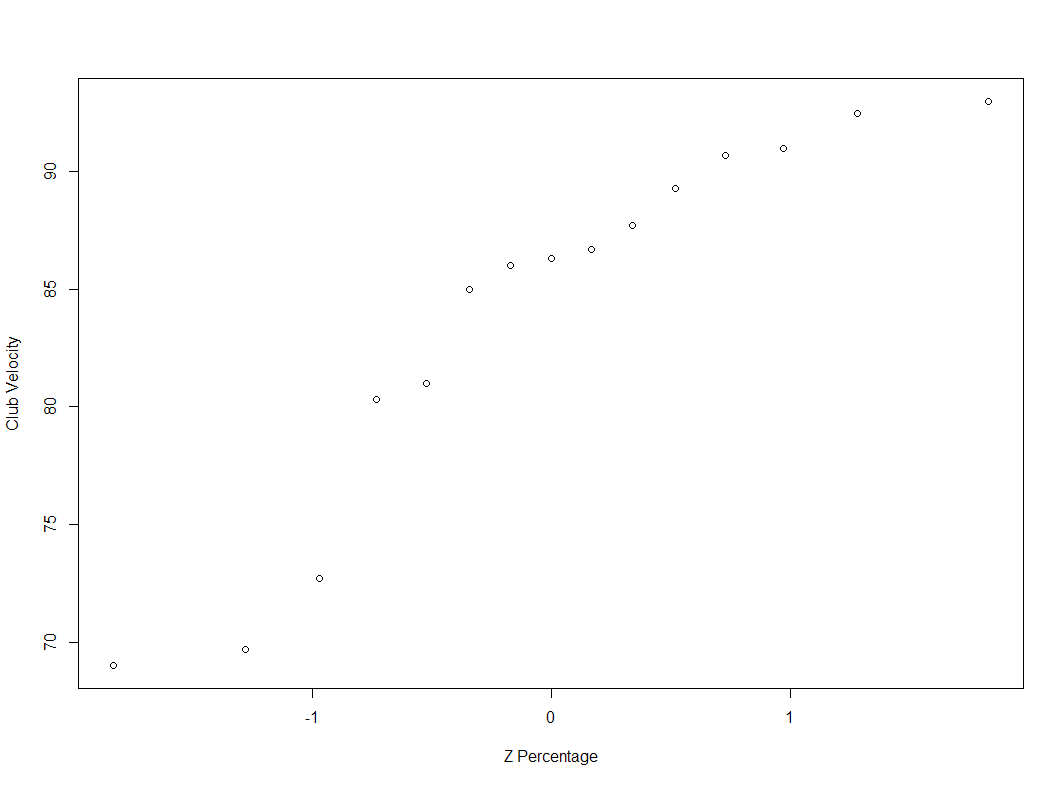
\includegraphics[width = \textwidth]{Rplot.png}
\end{center}
Looking at the plot we can see some slight skew, especially in the lower percentiles, however in large part the majority of the data looks to be normally distributed. 
\end{exercise}
\vspace{.5in}








\begin{exercise}{5.4} Return to the situation...
  \begin{enumerate}
    \item Determine the marginal pmf of $X_1$, and then calculate the  expected  number  of  customers  in  line  at  the  express checkout.
    \solution Fist we proceed by calculating the marginal pmf for $X_1$ by summing over the values of the table, row wise,
    \begin{equation*}
      \begin{pmatrix}
        p_{X_1}(0) && .19\\
        p_{X_1}(1) && .3\\
        p_{X_1}(2) && .25\\
        p_{X_1}(3) && .14\\
        p_{X_1}(4) && .12 \\
        Otherwise && 0
      \end{pmatrix}.
    \end{equation*}
Now we compute the expected value like any other discrete random variable (here it is as a dot product), 
\begin{equation*}
  E(X_1) =      
   \begin{pmatrix}
    .19\\
    .3\\
    .25\\
    .14\\
    .12
  \end{pmatrix} \cdot
  \begin{pmatrix}
    0\\
    1\\
    2\\
    3\\
    4
  \end{pmatrix} = 1.7
\end{equation*}

\vspace{.25in}

\item  Determine the marginal pmf of $X_2$\\

\solution  Calculating the marginal pmf for $X_2$ by summing over the values of the table, column wise,
\begin{equation*}
  \begin{pmatrix}
  p_{X_2}(0) && p_{X_2}(1) && p_{X_2}(2) && p_{X_2}(3) && Otherwise\\
  .19 && .3 && .28 && .23 && 0
\end{pmatrix}
\end{equation*}

\vspace{.25in}

\item By   inspection   of   the   probabilities   $P(X_1 = 4)$, $P(X_2 = 0)$,  and $P(X_1 = 4, X_2 = 0)$,  are  $X_1$  and  $X_2$ independent random variables? Explain.\\
\solution Note that $P(X_1 = 4) = p_{X_1}(4) = .12$ and that $P(X_2 = 0) = p_{X_2}(0) = .19$. Consider that when variable are independent $P(X_1,X_2) = P(X_1)P(X_2)$ thus since,
\begin{equation*}
  p(4,0) = 0 \neq .12(.19) = p_{X_1}(4)P_{X_2}(0).
\end{equation*}  
Thus the variables are dependent.
\end{enumerate}
\end{exercise}
\vspace{.5in}

\begin{exercise}{5.10}  "Annie and Alvie..." \\
  \begin{enumerate}
    \item What is the joint pdf of $X$ and $Y$?\\
    \solution Since the variables $X$ and $Y$ are stated to be independent we know that, $f(x,y) = f_x(x)f_y(y)$. We also know that the 
    marginal pdfs are uniform overthe support $5 \le x,y \le 6$ which is an interval size 1. Thus,
    \begin{equation*}
      f(x,y) = 
      \begin{cases} 
        1 &  5 \le x,y \le 6\\
        0 & Otherwise 
     \end{cases}.
    \end{equation*}
    \vspace{.25in}


    \item What is the probability that they both arrive between 5:15 and 5:45?\\
    \solution First recognize that 15 minutes is a quarter of an hour, and it follows that 45 minutes is 3 quarters of an hour, 
    thus what we mean to solve is $P(5.25 \le X,Y \le 5.75)$. Since the variable are independent we can calculate the joint probability by multiplying together the marginal probability,
    \begin{equation*}
      P(5.25 \le X \le 5.45) = \int_{5.25}^{5.45} 1 dx  = .5
    \end{equation*}
    \begin{equation*}
      P(5.25 \le Y \le 5.45) = \int_{5.25}^{5.45} 1 dy  = .5
    \end{equation*}
    Thus we get the following,
    \begin{equation*}
      P(5.25 \le X,Y \le 5.75) = .5(.5) = .25
    \end{equation*}
    \vspace{.25in}






    \item Integrate the joint pdf over this area $A = \{(x,y):|x - y|\le 1/6\}$\\
    
    \solution First sketching area that we are going to integrate over, note that in this sketch its the area between the black lines contained by the support of the joint pdf,
    \begin{center}
      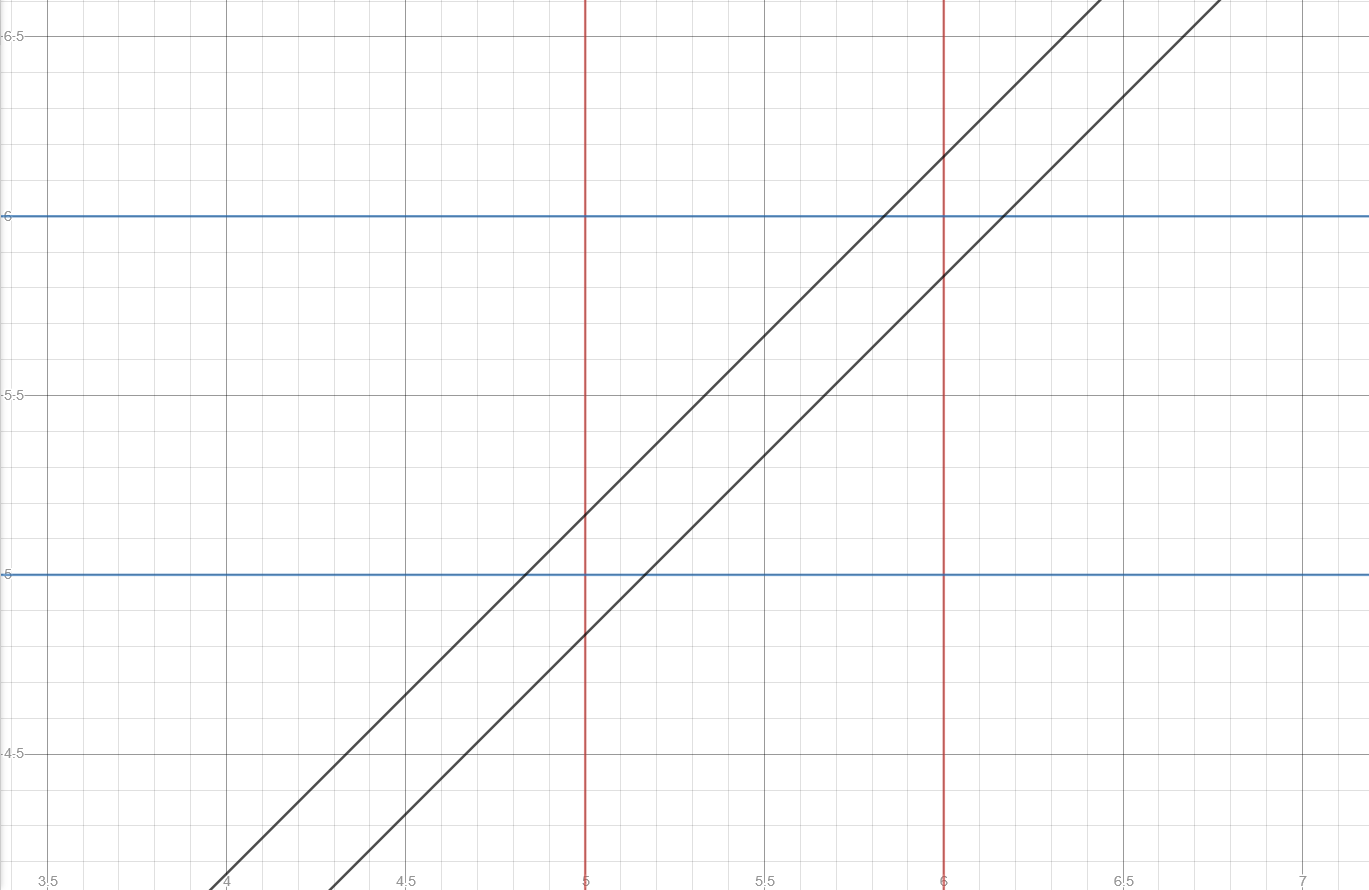
\includegraphics[width = \textwidth]{plotsketch.png}
    \end{center}
    Taking advantage of symmetry and compliments we can calculate the probability,
    \begin{equation*}
      P((X,Y) \in A) = P((X,Y)) - P((X,Y)\notin A).
    \end{equation*}
    Consider the following double integral,
    \begin{equation*}
      \int _5^6\:\int _5^6\:1dydx-2\left(\int _{5+\frac{1}{6}}^6\:\int _5^{x\:-\:\frac{1}{6}}\:1dydx\right) = \dfrac{11}{36}
    \end{equation*}
    The first part integrates over the whole support and the second integrates over the values $(x,y) \notin A$.
  \end{enumerate}
\end{exercise}













\end{document}